% $Id: circuit.tex 8323 2020-11-18 02:26:39Z mskala $

%
% MSK 014 circuit explanation
% Copyright (C) 2022  Matthew Skala
%
% This program is free software: you can redistribute it and/or modify
% it under the terms of the GNU General Public License as published by
% the Free Software Foundation, version 3.
%
% This program is distributed in the hope that it will be useful,
% but WITHOUT ANY WARRANTY; without even the implied warranty of
% MERCHANTABILITY or FITNESS FOR A PARTICULAR PURPOSE.  See the
% GNU General Public License for more details.
%
% You should have received a copy of the GNU General Public License
% along with this program.  If not, see <http://www.gnu.org/licenses/>.
%
% Matthew Skala
% https://northcoastsynthesis.com/
% mskala@northcoastsynthesis.com
%

\chapter{Circuit explanation}

The Gracious Host is a digital module and most of its features are
implemented in firmware.  There is another entire volume, the \emph{MSK~014
Gracious Host Programmer's Manual}, describing how the firmware works.  That
leaves very little to be said about the hardware as such.  But here are a
few comments about the circuit, especially concentrating on the analog parts.

\section{Digital parts and power}

Most of the intelligence in the module is inside a Microchip PIC24FJ64GB002
microcontroller chip.  This is basically a complete 16-bit microcomputer on
a chip with 8K of built-in RAM, a bunch of peripheral devices, and 64K of
built-in flash memory used to store the firmware.  Kits and built modules
come with preprogrammed chips (possibly not the very latest version of the
firmware); new firmware can be loaded over the USB port.

There are a few other digital components directly wired to the relevant
ports on the microcontroller: a 4.000\,MHz clock oscillator; an MCP4822
12-bit two-channel DAC; and a 23LC1024 serial RAM with a capacity of 128K. 
The oscillator provides accurate timing control, which is especially
required for USB communication.  The DAC controls the analog output jack
voltages.  The SRAM chip, in the current firmware, is used as a buffer
during firmware upgrades; it is also available for use by future and
third-party firmware which may need more than the microcontroller's built-in
8K RAM.

Pin~14 of the microcontroller is brought out to the test point P5 on the
back of the module.  With the standard build of the firmware, there is no
signal on this test point, but debugging code can send signals to this point
where they can be observed with an oscilloscope.

None of these digital components requires much in the way of support
circuitry beyond decoupling capacitors, including the extreme 10\,$\mu$F
ceramic cap on pin~20 of the microcontroller.  The digital components all
run on $+$3.3V power, regulated down from the Eurorack $+$5V supply by an
MCP1700-3302 LDO regulator.  The microcontroller actually uses a lower
voltage internally; that large capacitor is intended to support the
microcontroller's built-in regulator, which seems to be a switching type for
reasons of power economy.  The microcontroller also has a connection to the
$+$5V supply, to support the USB voltage requirements.

The power input is also straightforward.  The $\pm$12V rails have series
Schottky diodes to protect against reverse connection, although this is less
an issue on the Gracious Host with its 16-pin connector than would be the
case on a module with a 10-pin power connector.  Reversing the 16-pin
connector shorts the $+$5V and $+$12V lines into ground and will probably
cause the power supply to shut down relatively harmlessly.  The power rails
also have 10\,$\mu$F electrolytics to reduce general interference, though the
smaller per-chip decoupling caps will have a more significant effect.  The
$+$5V power rail has no Schottky diode because we cannot afford the voltage
drop, but it does go through a 200mA polyfuse, with a 150\,$\mu$F capacitor on
the far side, according to Microchip's recommended circuit for powering the
USB bus.

Except for the connections to the USB port, which have their own built-in
drivers and protective circuits, all the digital components are buffered from
the outside world by op amp circuits running on the Eurorack $\pm$12V
supply, which translate the levels and protect the digital components from
out-of-range voltages.  Those are discussed in more detail in the next few
sections.

\section{Analog input buffers}

Figure~\ref{fig:analog-in-buffer} shows the circuit for one of the input
jacks.  The same section is repeated for the other.

\begin{figure*}
{\centering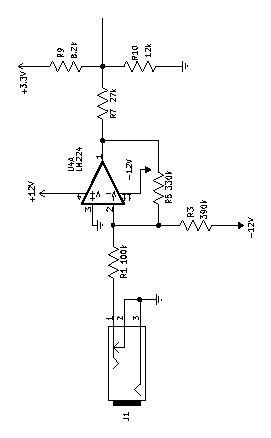
\includegraphics[scale=2,rotate=-90]{opamp1.eps}\par}
\caption{Analog input buffer.}\label{fig:analog-in-buffer}
\end{figure*}

This circuit is intended to serve two goals:  first, map the input range
0--5V (intended useful range of the input jacks) to be within 0--3.3V (the
measurement range of the microcontroller's built-in ADC); and second, make
sure that no voltage within $\pm$12V applied to the input jack can result in
a voltage applied to the microcontroller outside the range $-$0.3V to
$+$3.6V, representing the microcontroller's absolute maximum rating.  It
ought to achieve these goals in all conditions of component variation within
tolerance.  It also ought to present not too large an impedance to the
microcontroller input, because ADC conversion time suffers when the driving
impedance is too large.

The circuit topology is best understood working back from the
microcontroller input.  We could imagine that the op amp output might vary
over as much as $\pm$12V -- not really, because this op amp is not rail to
rail, but that is a conservative worst case.  No matter what goes on at the
input jack, we want the op amp to be unable to apply a damaging voltage to
the microcontroller.  The three-way voltage divider of R7, R9, and R10 is
designed to guarantee that no op amp output (divider input) voltage inside
$\pm$12V can result in a microcontroller input (divider output) voltage
outside $-$0.3 to $+$3.6V.  Also, the output impedance of the divider (which
will be equal to the parallel combination of the three resistors) ought to
be no more than about 5k$\Omega$, for compatibility with the ADC's drive
requirements.

I selected the divider resistor values mostly by trial and error with a
simulator.  But a rough calculation to guide such experiments proceeds by
simplifying the circuit:  instead of a three-resistor divider between the op
amp at $\pm$12 and the 0V and 3.3V rails, we can think of it as a
two-resistor divider between the op amp and \emph{some unspecified constant
voltage to be chosen later}.  The resistors R9 and R10 are replaced by their
equivalent circuit.  Then it's easier to analyse.  One side of the
divider is R7, and the other is the parallel combination of R9 and R10
$(\textrm{R}9\|\textrm{R}10)$, which I will call RX.

Knowing that we need the 24V input range to map to at most a 3.9V output
range means the gain through this divider can be at most $3.9/24$, about
0.162; and then R7/RX should be at least about $(1-0.162)/0.162=5.17$. 
Combining that with the target of R7$\|$RX$=$5k$\Omega$ (desired output
impedance) we can write out the equations and solve them to get starting
estimates of R7$=$30.85k$\Omega$ and RX$=$5.97k$\Omega$.  None of this
depends on knowing the constant voltage on the other side of the
two-resistor divider.

The next step is to get a target for that constant voltage.  If we decide
$+$12V input should map to $+$3.6V output, then Ohm's law with the tentative
value of R7 says that the 30.85k$\Omega$ resistor, dropping
12V$-$3.6V$=$8.4V, will carry 272$\mu$A.  That much current through RX with
the tentative value of 5.97k$\Omega$ gives a voltage drop across RX of 1.62V
from the 3.6V output value, and the other end of RX is at 1.98V.

Now we choose values for R9 and R10, connected to $+$3.3V and 0V
respectively, such that their combination will be equivalent to a single
5.97k$\Omega$ resistor connected to 1.98V.  Dividing $1.98/3.30=0.600$
indicates that $\textrm{R}10/(\textrm{R}9+\textrm{R}10)$ should be close to
0.600.  Combining that with R9$\|$R10$=$RX$=$5.97k$\Omega$ and solving gives
estimates R9$=$9.95k$\Omega$, R10$=$14.92k$\Omega$.  Those and the earlier
value R7$=$30.85k$\Omega$ are reasonable starting points for simulator
experiments.  I started with standard values near there, simulated the
input/output function in Qucs, and tweaked the values until I got results
that looked reasonable.  I ended up with all three resistor values a little
smaller than these estimates, presenting a slightly lower impedance to the
ADC.

Choosing the resistors around the op amp (R1, R3, and R5) was simpler
because of fewer interactions between them.  Wanting to have a typical
Eurorack input impedance of 100k$\Omega$ dictated the value of R1 as
100k$\Omega$.  Although I calculated the divider downstream on the
assumption that the op amp might produce any voltage in $\pm$12V, really I
only think I can reliably expect it to swing over $\pm$10.3V.  That is a 12V
rail on each side, minus 0.2V eaten by the reverse-protection diode,
minus 1.5V to reflect the op amp's output swing capabilities (probably
better than that on the negative side but this is the specification for the
positive side and I am conservatively assuming the same on both sides).  So
this circuit should be free of clipping on a 5V input range if it maps it to
a 20.6V output range, and that means the magnitude of the amplifier's
negative gain should be no more than 20.6V$/$5V$=$4.12; R5 should be no more
than 412k$\Omega$, and probably near that much.  Then R3 should be whatever
it takes to shift the 0--5V input range to something that, when seen through
the downstream voltage divider, will be comfortably within the
microcontroller's 0--3.3V measurement range.

I did not bother to calculate a precise estimate for R3 but went directly to
the simulator and tried different standard values for it and R5 until I
found some that seemed to work well.  The op amp gain ended up smaller than
estimated above partly because 20.6V is actually a little too wide as the
output range from the op amp: the downstream voltage divider is designed to
map all possible op amp voltages to a \emph{non-damaging} range of 3.9V, but
we need 0--5V at the input jack to map to the \emph{measurable} range of
3.3V, and do it in all possible conditions of component tolerances, and
given the use of convenient standard values for the components instead of
exactly calculated ones.  There is also some interaction and compromise
between the offsets introduced by R3 and by the R9/R10 voltage divider. 
Playing with different standard values until all the voltages worked out in
simulation eventually gave the choices shown on the schematic.

\section{LED drivers}

The LED driver section is as shown in Figure~\ref{fig:led-driver}.  It is
repeated on both sides, sharing the voltage divider of R13 and R14.

\begin{figure*}
{\centering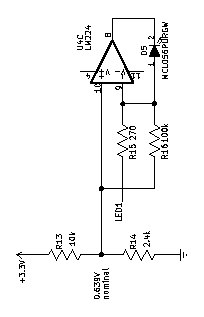
\includegraphics[scale=2,rotate=-90]{opamp2.eps}\par}
\caption{LED driver.}\label{fig:led-driver}
\end{figure*}

This circuit is driven by GPIO pins on the microcontroller, which have three
states:  high, $+$3.3V and able to source a lot of current; low,
0V and able to sink a lot of current; and high-impedance or tri-state, in
which the pin effectively disconnects from the circuit entirely, neither
sourcing nor sinking current.  The LED is a bi-colour unit, actually two
LEDs wired anti-parallel, so current in one direction will make it light up
red, and in the other direction, green.

We want to drive a controlled amount of current through the LED in each
direction, so that the brightness of each colour will be roughly equal. 
This is complicated a little by the fact that the LED will have different
luminous efficiency (brightness per milliamp) in each direction, and the
\emph{voltage} it takes to drive that current will vary with the direction,
individual LED unit, colour, temperature, and ambient light level, at least. 

Just connecting the LED between the GPIO pin and some constant voltage in
the middle of the 3.3V range would work if we could depend on consistent
forward voltages for the two colours, adding up to 3.3V.  Adding a series
resistor would help even out variations in the forward voltages, if we could
depend on the sum of LED forward voltages being significantly \emph{less}
than 3.3V.  But in fact, the forward voltages needed for red and green LEDs
are usually more like 2V each, so the microcontroller's output driver with a
3.3V swing cannot light the LED in both directions with such a simple
circuit.  Putting the LED between two GPIO pins, with a resistor to help
control the current, would double the voltage swing and might work but would
require more pins than are available.  There would also be issues with
controlling the current in the two directions separately.  So the Gracious
Host instead uses an op amp circuit that controls the current more precisely
and is capable of operating over a wider voltage range.  The driver
basically uses the ``connect GPIO pin to a constant voltage in the middle of
the range'' approach but it puts a well-behaved resistor there instead of
the LED, allowing the use of lower voltages, and then it echoes the current
through the resistor into the LED.

The resistor R15 is really the heart of the circuit:  it converts voltage to
current.  Op amps in negative feedback always act to bring their inputs to
equal voltage.  The R13/R14 voltage divider provides a basically constant
voltage (about 0.64V) to the positive input of the op amp, and then we can
assume that the negative input will be at 0.64V too.  When the GPIO pin is
high (3.3V), the voltage drop across R15 is 3.30V$-$0.64V$=$2.66V and the
current through R15 is 2.66V$/$270$\Omega=$9.85mA.  When the GPIO pin is low
(0V), the voltage drop across R15 is 0.64V \emph{in the other direction}. 
The current through R15 is $-$0.64V$/$270$\Omega=-$2.37mA.

These amounts of current flow through R15; but the total current into and
out of the op amp's negative input must be zero (Kirchoff's Law and the high
impedance of the op amp input).  Effectively no current flows through R16
because of its high resistance compared to the components around it.  So all
the current through R15 must also be passing through the LED.  High and low
states of the microcontroller GPIO pin correspond to currents of $+$9.85mA
and $-$2.37mA through the LED.  The op amp will automatically adjust its
output voltage to get these currents, regardless of variations in the LED's
forward voltage.

The overall brightness of the LED is determined by the value of R15:  the
sum of (the absolute values of) the two currents is necessarily 3.3V$/$R15,
so we could make both colours brighter or dimmer by changing this resistor. 
The ratio of current for red and green is determined by the 0.64V voltage
applied to the op amp positive input, and therefore by the ratio of R13 and
R14.  Raising or lowering this voltage increases current in one colour state
and decreases it in the other.  The actual values I chose were determined by
experiment, starting with an estimate from the LED's data sheet values for
visible brightness in millicandelas at different current levels.  LEDs
within their normal operating range tend to be quite linear in brightness
relative to current.

But what about the high-impedance GPIO state, and R16?  When the GPIO pin
goes into the high-impedance state, we want the LED to turn off.  In that
case the GPIO pin is effectively disconnected, and so is R15.  There is no
current through R15 and the LED driver circuit, trying to match the R15
current through the LED as well, will basically put no current through the
LED -- as desired.

But although the current through the op amp's input is usually approximated
as zero, it isn't really.  Op amps always require a small \emph{bias
current} through their inputs, and for the LM224 in particular the bias
current is on the order of 20nA, a small amount of current in absolute terms
but actually relatively large for an op amp.  Bias current generally depends
on the type of op amp; bipolar-input units like the LM224 tend to have more
than other designs.  Some CMOS op amps designed specifically for ultra-low
bias current are able to achieve orders of magnitude less.  Without R16, the
op amp would try to bring its negative input to the same voltage as the
0.64V at the positive input, by driving the tiny bias current through D5. 
The bias current would not be enough to light the LED.

The problem is that LEDs tend to be unpredictable at such low current
levels, and op amps like this one are not really designed to produce
tightly-controlled very low current levels either.  The LED may end up
behaving more like a capacitor than a resistor; it may also generate a small
voltage of its own by converting ambient light into electricity, in an
effect similar to what a solar cell does.  What the op amp needs to do to
drive 20nA through the LED will vary moment by moment and it may end up
being unstable.  In practice it would \emph{probably} work fine anyway, but
I wanted to be on the safe side.

To make sure everything stays under control in the LED-off situation, the
resistor R16 ties the op amp inputs together, providing a path for the bias
current to the relatively low-impedance output of the R13/R14 voltage
divider instead of only through the LED.  With the LED on, the current
through the 270$\Omega$ resistor overwhelms the contribution of R16, which
distorts the current levels from their target values only by a tiny amount. 
But with the LED off, the current through R16 overwhelms the unstable
contribution of whatever comes through the even higher impedance of the LED. 
Limiting the impedance at the negative input to 100k$\Omega$ means the op
amp can drive its output, and the far side of the LED, to 0.64V without
needing to operate in the very low current range where it may not function
well.

\begin{figure*}
{\centering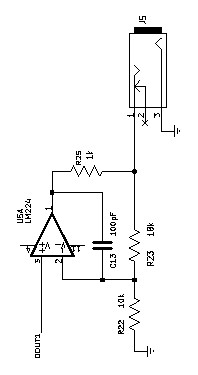
\includegraphics[scale=2,rotate=-90]{opamp3.eps}\par}
\caption{Output buffer.}\label{fig:out-buffer}
\end{figure*}

\section{Output buffers}

The output driver section is shown in Figure~\ref{fig:out-buffer}.  All four
output jacks use this circuit.  The digital output buffers take their input
from microcontroller GPIO pins, and the analog output buffers take their
input from the DAC outputs.  The GPIO pins have low and high states of 0V
and 3.3V, which the output buffer circuit amplifies to 0V and a little over
9V.  The DAC outputs (in the mode normally used) have a range of 0V to
2.048V, which the output buffer amplifies to a nominal range of 0V to 5V
with a little extra margin available at the top (calculated limit 5.73V).

This is a reasonably straightforward non-inverting op amp amplifier circuit
with a voltage gain of 2.8 and a couple of components added to improve
stability.  Ignoring R25 and C13 for the moment, R22 and R23 form a voltage
divider that divides the output voltage as seen at the jack, by 2.8.  The op
amp in negative feedback always acts to make its inputs equal.  So for any
given voltage coming into this section along the wire labelled DOUT1, the op
amp will bring its own output voltage to whatever voltage causes the output
jack to be at 2.8 times the DOUT1 voltage.  As long as the op amp is capable
of doing that, the section has an overall gain of 2.8.  Input of 0V gives
output of 0V; input of 3.3V gives output of 9.24V; and input of 2.05V gives
output of 5.73V.

But there can be some issues with a very simple op amp circuit, usually
related to what happens if the user plugs something weird into the jack
socket.  In particular, if the op amp's output is \emph{directly} connected
to the jack socket and the user plugs in a short circuit, or another output
similarly designed, then the op amp may attempt to drive the jack to a
voltage that the external connection will not allow.  The op amp will just
dump more and more current into the conection, trying to raise the voltage. 
In principle, that kind of overload can be damaging.  This particular op amp
has built-in protection against such situations, so it probably will not
damage \emph{itself}, but the high current could be damaging to whatever is
on the other end of that cable, and it could indirectly cause problems by
overloading power supplies, etc.  Adding R25 limits how much current the op
amp will be able to source or sink through the jack in an overload
situation.

Another, subtler, issue has to do with stability.  Suppose the user plugs
something into the jack socket that exhibits significant capacitance.  A
very long patch cable would be an example.  Capacitive loads are in a sense
slow to respond to current.  If the input goes high and the op amp tries to
raise the voltage to match, the current flowing into the cable capacitance
may require some nonzero time to charge the capacitance and really raise the
voltage.  So the op amp continues trying to raise the voltage even after the
point at which it should have turned off its output current.  Then the
voltage ends up too high when things start to settle down, and so the op amp
is forced to draw current in the other direction to lower the voltage, and
it can overshoot there as well.  Mild overshoots that die down after a few
cycles are called \emph{ringing} and result in the voltage bouncing around a
little before settling down, every time it changes.  In more extreme cases,
a larger amount of cable capacitance can set up a self-sustaining
\emph{parasitic oscillation}, in which the op amp produces a continuously
changing voltage that never settles down, usually over its entire output
range with a frequency in the hundreds of kHz to a few MHz.

The resistor R25 helps prevent ringing and parasitic oscillation by limiting
how strongly the op amp can apply current to the external connection, and
therefore the extent of a possible quick overshoot.  The capacitor C13 also
helps, by inhibiting the op amp's gain at high frequencies.  Capacitors have
lower impedance as the frequency goes higher, so at the high frequencies
associated with these instability phenomena, C13 applies extra negative
feedback, reducing the gain below the level where temporary or sustained
oscillation would be possible.  At lower frequencies, the impedance of C13
is so high as to have little or no effect on circuit operation.  The effect
of C13 can also be stated in terms of its applying a phase shift that keeps
the circuit away from the region on a phase and gain versus frequency plot
where oscillation would be an issue.
